\section{Model Validation Diagnostics}
\label{app:model-diagnostics}

This appendix provides the detailed confusion matrices corresponding to the
training-only supervised and unsupervised model comparisons discussed in
Section \ref{sec:evaluation}.

\subsection{Supervised out-of-fold comparison}

\begin{figure}[p]
    \centering
    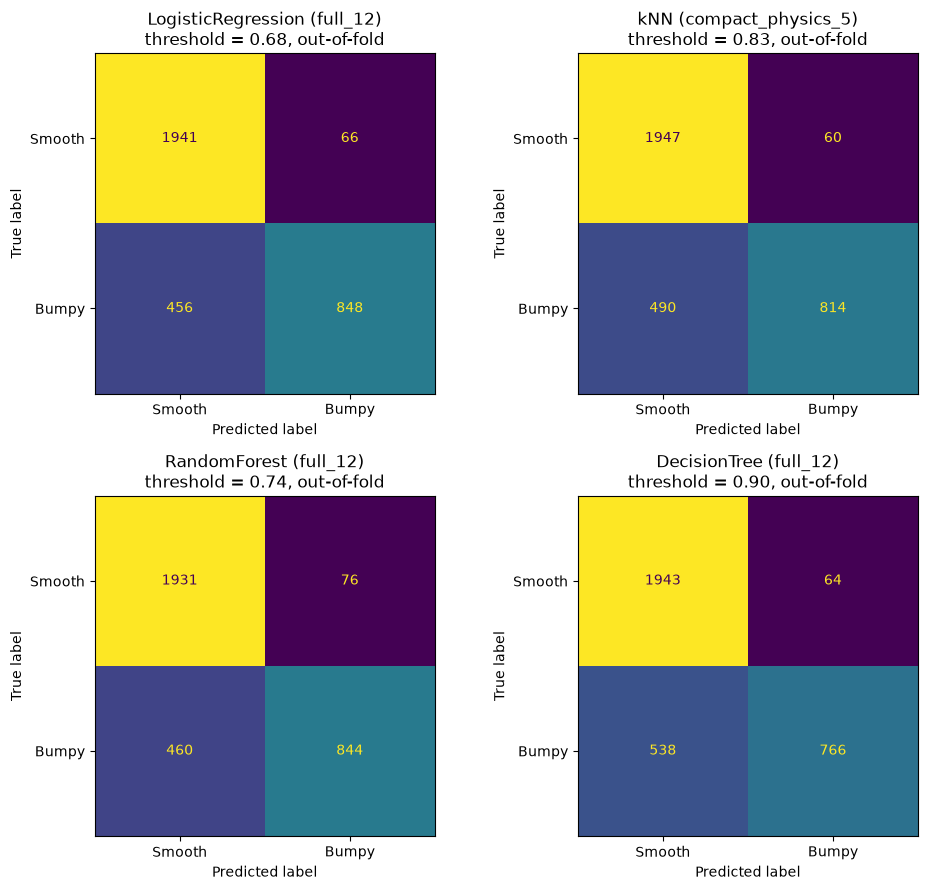
\includegraphics[width=\textwidth]
    {figures/confusion-matrices-supervised.png}
    \caption{Training-only out-of-fold confusion matrices for the best
    configuration from each supervised model family. The thresholds shown
    were selected using out-of-fold training predictions and were fixed before
    final held-out evaluation. Logistic Regression achieved the highest
    validation $F_{0.5}$ score and was therefore selected as the final model.}
    \label{fig:appendix-supervised-cm}
\end{figure}

Across the supervised candidates, all selected operating points favour a low
false-positive rate for Bumpy predictions. Logistic Regression provided the
best $F_{0.5}$ compromise, with 66 Smooth windows incorrectly classified as
Bumpy and 848 correctly detected Bumpy windows in the combined out-of-fold
training predictions.

\subsection{Unsupervised comparison}

\begin{figure}[p]
    \centering
    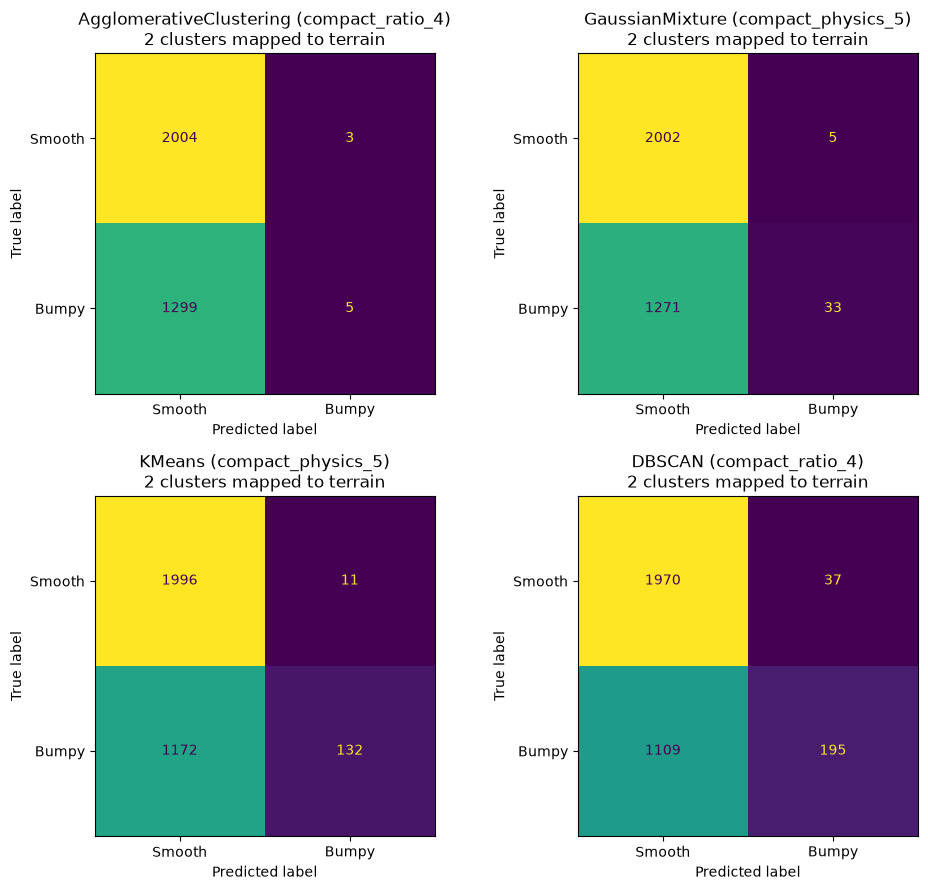
\includegraphics[width=\textwidth]
    {figures/confusion-matrices-UNsupervised.png}
    \caption{Mapped training-set confusion matrices for the best configuration
    from each unsupervised clustering family. Terrain labels were not used
    during clustering and were applied only afterwards to map clusters for
    diagnostic comparison.}
    \label{fig:appendix-unsupervised-cm}
\end{figure}

The mapped confusion matrices reinforce the distinction between internal
cluster separation and terrain-class agreement. Agglomerative Clustering and
Gaussian Mixture Modelling formed internally well-separated structures, but
these structures mapped predominantly to the Smooth class. DBSCAN produced
the greatest correspondence with the Smooth/Bumpy target among the evaluated
clustering methods, although its agreement remained weak compared with the
supervised approaches.

